\documentclass[12pt]{article}
\usepackage{amsmath,amssymb,amsfonts,amsthm,fullpage,setspace,float,graphicx}
\newtheorem{corollary}{Corollary}
\newtheorem{lemma}{Lemma}
\newtheorem{proposition}{Proposition}
\renewcommand{\qedsymbol}{$\blacksquare$}
\begin{document}
\noindent\textit{I've done the math enough to know the dangers of our second guessing.\\ Doomed to crumble unless we grow, and strengthen our communication.}\\ \\$\sim$ From ``Schism,'' by Tool. \\ \\
\noindent\textit{Uniform Noise, Quadratic Loss.} Set $L(x)=\frac{1}{2}x^2$. Fix $\bar{\epsilon}\in(0,1)$, and $I\in C^{1}[0,1]$. As they will appear frequently, put $I_{0}(s,t):=\int_{s}^{t}{\iota(r)dr}$, and $I_{1}(s,t):=\int_{s}^{t}{r\iota(r)dr}$. Actions are maps from received messages to actions: $\tilde{m}\mapsto a(\tilde{m})$. Messages are maps from states to sent messages: $q\mapsto m(q)$. We consider strictly increasing, piecewise twice continuously differentiable action and message functions. Formally, define
\begin{align}
\mathcal{A}&:=\{\alpha\in D^{2}[-\bar{\epsilon},1+\bar{\epsilon}]\:|\:\text{for all }q\in[-\bar{\epsilon},1+\bar{\epsilon}],\:\alpha'(q)>0,\text{ and }\alpha(q)\in(0,1)\},\text{ and}\\
\mathcal{M}&:=\{\mu\in D^{2}[0,1]\:|\:\text{for all }q\in[0,1],\:\mu(0)=0,\mu(1)=1,\mu'(q)>0,\text{ and }\mu(q)\in[0,1]\}.
\end{align}
to be the sets of admissable action and message functions respectively. Note that the receiver's action has domain $[-\bar{\epsilon},1+\bar{\epsilon}]$. The sender's message has codomain $[0,1]$, but it is corrupted by noise. Although a \textit{sent} message may be no smaller than zero, and no larger than one, a \textit{received} message may be as small as $-\bar{\epsilon}$, or as large as $1+\bar{\epsilon}$. The receiver must choose an action in $[0,1]$ for messages less than zero or greater than one. The sender has ex-ante payoffs $S:\mathcal{A}\times\mathcal{M}\rightarrow\mathbb{R}$ given by
\begin{equation}
S(a,m)=\frac{1}{2\bar{\epsilon}}\int_{-\bar{\epsilon}}^{\bar{\epsilon}}{I(q)L(a(m(q)+e)-q)g(q)de}
\end{equation}
\textit{Beliefs.} Let $g(q\:|\:\tilde{m})$ denote the receiver's beliefs. Put $\tilde{m}=m(q)+e$, where $e\sim U[0,1]$. Define the upper and lower limits to be 
\begin{align}
\overline{q}(\tilde{m})&=m^{-1}(\min\{\tilde{m}+\bar{\epsilon},1\}),\text{ and}\\
\underline{q}(\tilde{m})&=m^{-1}(\max\{\tilde{m}-\bar{\epsilon},0\})
\end{align} 
respectively. Now $\tilde{m}|q\sim U[m(q)-\bar{\epsilon},m(q)+\bar{\epsilon}]$. By Baye's Law,
\begin{equation}
g(q|\tilde{m})=\frac{f(\tilde{m}|q)}{\int_{0}^{1}{f(\tilde{m}|t)g(t)dt}}=\frac{\frac{1}{2\bar{\epsilon}}\mathbf{1}_{m(q)-\bar{\epsilon}\leq\tilde{m}\leq m(q)+\bar{\epsilon}}}{\int_{0}^{1}{\frac{1}{2\bar{\epsilon}}\mathbf{1}_{\underline{q}(\tilde{m})\leq t\leq\overline{q}(\tilde{m})}dt}}=\frac{\mathbf{1}_{\underline{q}(\tilde{m})\leq q\leq\overline{q}(\tilde{m})}}{\overline{q}(\tilde{m})-\underline{q}(\tilde{m})}
\end{equation}
The sender has ex-ante payoffs $R:\mathcal{A}\times\mathcal{M}\rightarrow\mathbb{R}$ given by
\begin{equation}
R(a,m,\tilde{m})=\int_{0}^{1}{I(q)L(a(\tilde{m})-q)g(q|\tilde{m})dq}.
\end{equation}
Next, we change the order of integration, first integrating with respect to $q$, then integrating with respect to $\tilde{m}$. Proceeding with the change of variables, we obtain 
\begin{equation}
J(a,m)=\int_{-\bar{\epsilon}}^{1+\bar{\epsilon}}{\int_{\underline{q}(\tilde{m})}^{\overline{q}(\tilde{m})}{{I(q)L(a(\tilde{m})-q)dq}d\tilde{m}}}.
\end{equation}
We have omitted the density of the noise, as it is constant, and therefore does not affect the equilibrium message and action functions. The \textit{sender and receiver's problem} is to choose $(a,m)\in\mathcal{A}\times\mathcal{M}$, which minimizes $J(a,m)$. Partition $[0,1]$ into the subsets $\{0\}$, $\mathcal{R}_{1}:=(0,\bar{\epsilon})$, $\mathcal{R}_{2}:=[\bar{\epsilon},1-\bar{\epsilon}]$, $\mathcal{R}_{3}:=(1-\bar{\epsilon},1)$, and $\{1\}$. We first show that there exists a unique solution to the sender and receiver's problem. We then show that steepness of the message function is increasing with the importance of getting the message right.
\begin{lemma}\label{lemma:message}
Given an action $a\in\mathcal{A}$, the sender's optimal message is.
\end{lemma}
\begin{proof}
Suppose that $(a,m)\in\mathcal{A}\times\mathcal{M}$ is a solution to the sender and receiver's problem. We proceed by enumerating the conditions that must be met by a pair $(a,m)$, and that $(a,m)$ is unique among them. If the received message is $-\bar{\epsilon}$, then the sent message was $0$ a.s., and hence the state of the world is also $0$. Therefore, it is optimal for the receiver to play $0$. If the received message is $1+\bar{\epsilon}$, then the sent message was $1$ a.s., and hence the state of the world is also $1$. Therefore, it is optimal for the receiver to play $1$. We have established that $a(-\bar{\epsilon})=0$, and $a(1+\bar{\epsilon})=1$. $(a,m)$ must satisfy the first-order condition with respect to $m$:
\begin{equation}
0=\int_{-\bar{\epsilon}}^{\bar{\epsilon}}{L'(a(m+e)-q)a'(m+e)de}=L(a(m+\bar{\epsilon})-q)-L(a(m-\bar{\epsilon})-q).
\end{equation}
Since $L$ is even, there are two solutions: $a(m+\bar{\epsilon})=a(m-\bar{\epsilon})$, and $a(m+\bar{\epsilon})-q=-(a(m-\bar{\epsilon})-q)$. The first implies that $a$ is constant, and hence $a\not\in\mathcal{A}$, which contradicts our assumption that $a\in\mathcal{A}$. Let $F:[0,1]^2\rightarrow\mathbb{R}$ be given by
\begin{equation}
F(q,m)=a(m+\bar{\epsilon})+a(m-\bar{\epsilon})-2q. 
\end{equation}
Note that the domain of the last argument is $[0,1]$, and \textit{not} $\mathcal{M}$. Now 
\begin{equation}
F_{m}(q,m)=a'(m+\bar{\epsilon})+a'(m-\bar{\epsilon})>0. 
\end{equation}
Lastly, observe that $m'=-(F_{m})^{-1}F_{q}>0$. The first-order condition with respect to $a$, requires a change of coordinates. Figure \ref{figure:region} illustrates this change in the order of integration. $(a,m)$ must satisfy the first-order condition with respect to $a$:
\begin{equation}
0=\int_{\underline{q}(\tilde{m})}^{\overline{q}(\tilde{m})}{I(q)L'(a-q)dq}\:\Rightarrow\:a(\tilde{m})=\frac{I_{1}(\overline{q}(\tilde{m}),\underline{q}(\tilde{m}))}{I_{0}(\overline{q}(\tilde{m}),\underline{q}(\tilde{m}))}
\end{equation}
Observe that
\begin{align}
2q&=\frac{I_{1}(\overline{q}(m(q)+\bar{\epsilon}),\underline{q}(m(q)+\bar{\epsilon}))}{I_{0}(\overline{q}(m(q)+\bar{\epsilon}),\underline{q}(m(q)+\bar{\epsilon}))}-\frac{I_{1}(\overline{q}(m(q)-\bar{\epsilon}),\underline{q}(m(q)-\bar{\epsilon}))}{I_{0}(\overline{q}(m(q)-\bar{\epsilon}),\underline{q}(m(q)-\bar{\epsilon}))}\\
&=\frac{I_{1}(m^{-1}(\min\{m(q)+2\bar{\epsilon},1\}),m^{-1}(\min\{m(q),1\}))}{I_{0}(m^{-1}(\min\{m(q)+2\bar{\epsilon},1\}),m^{-1}(\min\{m(q),1\}))}-\frac{I_{1}(m^{-1}(\max\{m(q),0\}),m^{-1}(\max\{m(q)-2\bar{\epsilon},0\}))}{I_{0}(q,m^{-1}(\max\{m(q)-2\bar{\epsilon},0\}))}\\
&=\frac{I_{1}(m^{-1}(\min\{m(q)+2\bar{\epsilon},1\}),q)}{I_{0}(m^{-1}(\min\{m(q)+2\bar{\epsilon},1\}),q)}-\frac{I_{1}(q,m^{-1}(\max\{m(q)-2\bar{\epsilon},0\}))}{I_{0}(m^{-1}(\max\{m(q),0\}),m^{-1}(\max\{m(q)-2\bar{\epsilon},0\}))}
\end{align}
Let $\mathcal{T}:C^{2}[0,1]\rightarrow C^{2}[0,1]$ be given by
\begin{equation}
[\mathcal{T}\ell](\tilde{m})=\frac{1}{2}\left(\frac{I_{1}(\ell(\min\{\tilde{m}+2\bar{\epsilon},1\}),\ell(\tilde{m}))}{I_{0}(\ell(\min\{\tilde{m}+2\bar{\epsilon},1\}),\ell(\tilde{m}))}+\frac{I_{1}(\ell(\tilde{m}),\ell(\max\{\tilde{m}-2\bar{\epsilon},0\}))}{I_{0}(\ell(\tilde{m}),\ell(\max\{\tilde{m}-2\bar{\epsilon},0\}))}\right).
\end{equation}
\textit{Example:} $I\equiv1$. $I_{1}(s,t)/I_{0}(s,t)=(s+t)/2$, which implies that
\begin{equation}
2\ell(\tilde{m})=\ell(\min\{\tilde{m}+2\bar{\epsilon},1\})+\ell(\max\{\tilde{m}-2\bar{\epsilon},0\}).
\end{equation}
There are three cases:
\begin{enumerate}
\item $\tilde{m}\in(0,2\bar{\epsilon})$: $\ell(x)=2^{x/2\bar{\epsilon}}$.
\item $\tilde{m}\in(2\bar{\epsilon},1-2\bar{\epsilon})$: $\ell(x)=x$. 
\item $\tilde{m}\in(1-2\bar{\epsilon},1)$: 
\begin{equation}
\ell(x)=1+\frac{2\bar{\epsilon}}{\log(2)}\left(2^{-\frac{1}{2\bar{\epsilon}}}-2^{-\frac{x}{2\bar{\epsilon}}}\right)
\end{equation}
\end{enumerate} 
\end{proof}
\begin{lemma}
Given a message $m\in\mathcal{M}$, the receiver's optimal action is.
\end{lemma}
\begin{proposition}
There is a unique equilibrium $(a,m)\in\mathcal{A}\times\mathcal{M}$. 
\end{proposition}
Next, we show that. We assume that the zeros of $I'$ are isolated: for each $q_{0}\in[0,1]$ satisfying $I'(q_{0})=0$, there is a neighborhood $\mathcal{U}$ of $q$ such that for all $q\in\mathcal{U}\setminus\{q_{0}\}$, $I'(q)\neq0$. If $I$ is analytic, then its zeros are isolated. 
\begin{corollary}
The steepness of the message function is increasing with the importance.
\end{corollary}
\begin{proof}
Let $(a,m)\in\mathcal{A}\times\mathcal{M}$ be the unique solution of the sender and receiver's problem. Choose $q\in(0,1)$ at which $I'(q)\neq0$ (so long as $I$ is non-constant, there is at least one such $q$). Let $F$ be as in the proof of Proposition \ref{proposition:main}. Since $m'=-(F_{m})^{-1}F_{q}$, $F_{qq}=0$, $F_{mm}>0$, and $F_{qm}=0$, we have that
\begin{equation}
m''=-(F_{m})^{-2}((F_{qq}+F_{qm}m')F_{m}-F_{q}(F_{mq}+F_{mm}m'))=(F_{m})^{-2}F_{q}F_{mm}m'>0.
\end{equation}
By the inverse function theorem, $I$ inverts on $\mathcal{U}$. We conclude that, 
\begin{equation}
\frac{dm'}{dI}=\frac{dm'}{dq}\frac{dq}{dI}>0
\end{equation}
as desired.
\end{proof}
\pagebreak
\begin{figure}[H]
\begin{center}
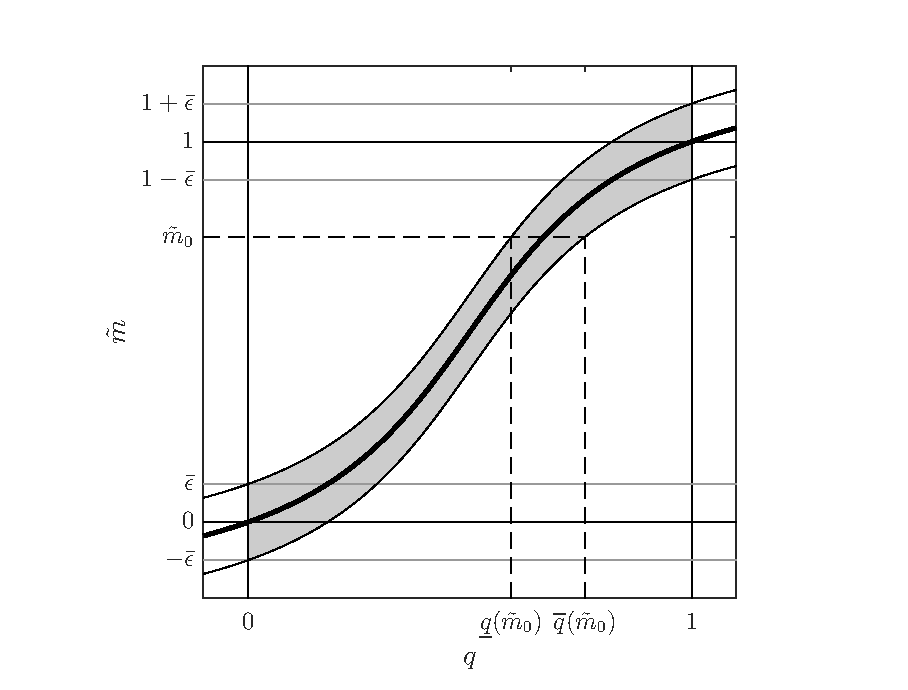
\includegraphics{region}
\end{center}
\caption{\textbf{The Region of Integration.} The solid line is $m(q)$, the upper dashed line is $m(q)+\bar{\epsilon}$, and the lower dashed line is $m(q)-\bar{\epsilon}$. The shaded area is the region of integration.}
\label{figure:region}
\end{figure}
\end{document}